
\documentclass{beamer}

\mode<presentation> {
\usetheme{Warsaw}
}

\usepackage{graphicx}
\usepackage{booktabs}
\usepackage{listings}
\usepackage{color}
\usepackage{hyperref}
\usepackage[lofdepth,lotdepth]{subfig}
\usepackage{hyperref}
\usepackage{fontawesome}

\definecolor{codegreen}{rgb}{0,0.6,0}
\definecolor{codegray}{rgb}{0.5,0.5,0.5}
\definecolor{codepurple}{rgb}{0.58,0,0.82}
\definecolor{backcolour}{rgb}{0.95,0.95,0.92}

\lstdefinestyle{mystyle}{
    backgroundcolor=\color{backcolour},   
    commentstyle=\color{codegreen},
    keywordstyle=\color{magenta},
    numberstyle=\tiny\color{codegray},
    stringstyle=\color{codepurple},
    %basicstyle=\footnotesize,
    basicstyle=\scriptsize\ttfamily,
    breakatwhitespace=false,         
    breaklines=true,                 
    captionpos=b,                    
    keepspaces=true,                 
    numbers=left,                    
    numbersep=5pt,                  
    showspaces=false,                
    showstringspaces=false,
    showtabs=false,                  
    tabsize=2,
    language=bash
}
 
\lstset{style=mystyle}

% \newcommand{\SubItem}[1]{
%     {\setlength\itemindent{15pt} \item[-] #1}
% }

%------------
%	TITLE PAGE
%------------

\title[Version control, Git and GitHub]{Introduction to Git - Practical session} 
\author{Criscely Luj\'{a}n}
\institute[Universit\'{e} Paris-Sud, UMR MARBEC]  
{Universit\'{e} Paris-Sud, UMR MARBEC \\ 
\medskip
\textit{criscely.lujan@ird.fr}}
\date{April 11, 2019}

\begin{document}

%------------
\begin{frame}
\titlepage 
\begin{center}

\includegraphics[height=1.5cm]{img/logo_psud.jpg}
\hspace{1em}

\includegraphics[height=1.5cm]{img/logo_marbec.png}
\hspace{1em}

\includegraphics[height=1.5cm]{img/logo_ird.png}
\end{center}
\end{frame}


\begin{frame}
\frametitle{GitHub account}

Tips about the name account:

\begin{itemize}
    \item Use your actual name!
    \item Shorter is better than longer!
    \item Be as unique as possible!
    \item Re-use your name from other context, e.g. \faTwitter, \faSlack, !
\end{itemize}
\end{frame}


\begin{frame}[fragile]
\frametitle{Git is already installed?}

To check that go to shell (terminal / command line / console) and enter \textbf{which git} to request the path to your Git executable:
\vspace{1em}

\begin{lstlisting}
which git
\end{lstlisting}

\vspace{1em}

Then enter \textbf{git --version} to see its version:

\begin{lstlisting}
git --version
\end{lstlisting}

\vspace{1em}

If git is not installed YET: See \href{https://happygitwithr.com/install-git.html}{\faStar Install git} to follow the correct steps to install git according your system operative! :)
\end{frame}


\begin{frame}[fragile]
\frametitle{Introduce yourself to Git}

Let \textbf{git} to know about you, following this simple configuration steps!
\vspace{1em}

\begin{lstlisting}
# Example
git config --global user.name "Criscely Lujan"
git config --global user.email "criscelylujan@gmail.com"
git config --global core.editor vim
git config --global --list
\end{lstlisting}

\vspace{1em}

\begin{itemize}
\item \textbf{user.name} can be your username. Your commits will be labelled with this name, so this should be informative!
\item \textbf{user.email} must be the email that you use to sign up for GitHub.
\item \textbf{core.editor} There are diverse options of \href{http://swcarpentry.github.io/git-novice/02-setup/}{\faStar Git editor}.
\end{itemize}
\end{frame}


\begin{frame}[fragile]
\frametitle{How authenticating yourself with GitHub}

There are two options of protocols for secure communication working over a computer network!

\vspace{1em}

1. \textbf{Hypertext Transfer Protocol Secure (HTTPS)}:

If you plan to work using HTTPS protocol, you can follow \href{https://happygitwithr.com/credential-caching.html#credential-caching}{\faStar \emph{Cache credential for HTTPS}} for more information.

\vspace{1em}
\vspace{1em}

2. \textbf{Secure Shell (SSH)}:

If you plan to work using SSH protocol, you can follow \href{https://happygitwithr.com/ssh-keys.html#ssh-keys}{\faStar \emph{Set up keys for SSH}} for more information.

\end{frame}


\begin{frame}
\frametitle{Git + RStudio + GitHub}

\begin{itemize}
    \item Tools, global options, Select Git/SVN tab.
    \item Create the RSA key.
    \item Click, view public key, and copy the displayed public key.
    \item Save the key on your GitHub account: Settings / SSH key / Add SSH key.
\end{itemize}

Step by step here: \href{https://www.r-bloggers.com/rstudio-and-github/}{\faStar Connecting RStudio and GitHub}.

\end{frame}


\begin{frame}
\frametitle{Make a new repository}

\begin{itemize}
    \item Go to GitHub and login. Click in the green box called \textbf{New repository}. 
    \item If you are on your own profile page, go to the section \textbf{Repositories}, then click the green box called \textbf{New}.
    \item Assign a name for the \textbf{repository} and include a \textbf{description} (this is optional but is recommended!).
    \item Public or private.
    \item Initialize the repository using the \textbf{README}.
\end{itemize}
\end{frame}

\begin{frame}[fragile]
\frametitle{Make a new repository}
\begin{center}
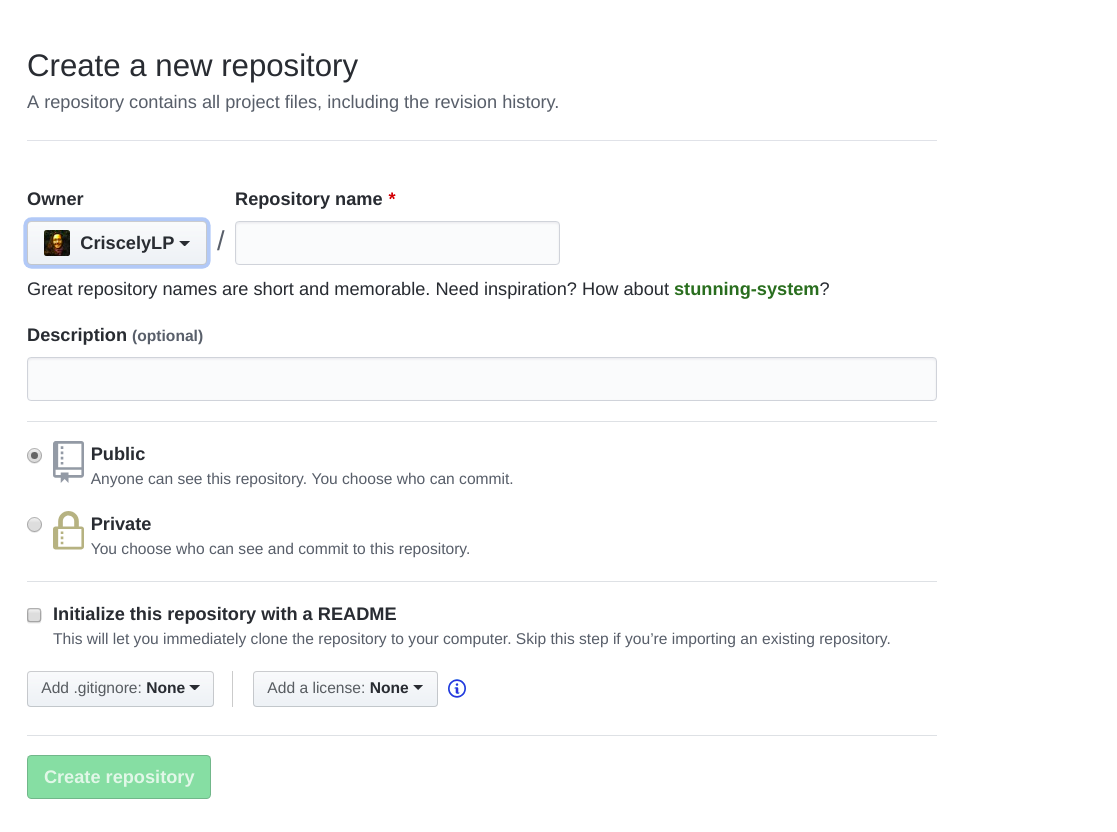
\includegraphics[scale=0.27]{img/github_makeRepo.png}
\end{center}
\end{frame}


\begin{frame}[fragile]
\frametitle{Clone a repository: Using RStudio}
\begin{itemize}
    \item File / New project. 
    \item Version control.
    \item Git.
    \item Fill \textbf{Repository URL} and project name (what you want the folder to be called locally).
\end{itemize}
\end{frame}

\begin{frame}[fragile]
\frametitle{Clone a repository: Using terminal}

- Create a new directory, open it and perform the following code:

\begin{lstlisting}
git init # to create a new git repository
\end{lstlisting}

- Clone the repository running the following command plus the path of the repository to be cloned:

\begin{lstlisting}
git clone git@github.com:umr-marbec/git-training.git #path used as example
\end{lstlisting}

This path is copied from the repository that we will be cloned.
\end{frame}


\begin{frame}[fragile]
\frametitle{Workflow}

Your local repository consists of three trees maintained by git.

\vspace{1em}
\begin{center}
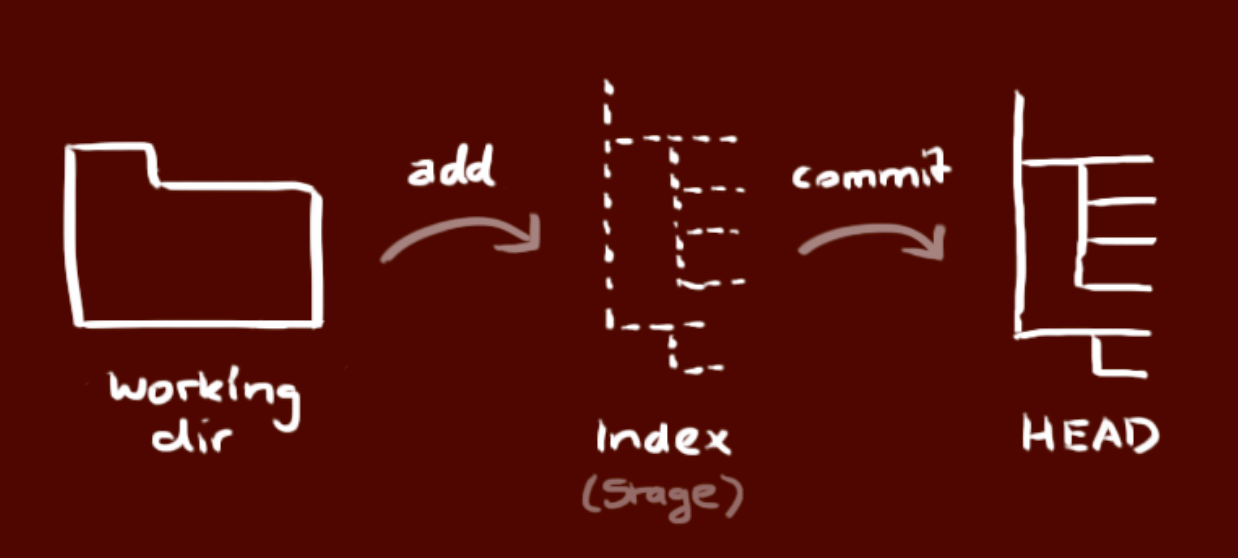
\includegraphics[scale=0.25]{img/workflow.png}
\end{center}
\end{frame}


\begin{frame}[fragile]
\frametitle{Add, commit and push}

- After clone the repository on your computer, you can make changes using \textbf{add}, \textbf{commit}, and \textbf{push}:

\begin{lstlisting}
git add <filename> # adding changes for specific file
git add . # adding all changes
git commit -m "Commit message" # changes commited to the HEAD
git push origin master #  changes to the remote repository (MASTER)
\end{lstlisting}

\end{frame}

\begin{frame}[fragile]
\frametitle{Exercise!!!}

\begin{itemize}
    \item Create a repository in GitHub.
    \item Clone the repository in your computer.
    \item Make changes (edit README.md and .gitignore).
    \item Make commits, if is possible include emojis to have fun! 
    \item Use: push / pull / merge / status / etc.
    \item Check the changes in you remore repository.
    \item Develop a new branch, delete it, play, and ... enjoy! \faSmileO
\end{itemize}


\end{frame}



\end{document}